\documentclass[final]{beamer}
\usepackage{etex}

\usepackage[scale=1.2]{beamerposter}

\usetheme{confposter}

% \newlength{\sepwid}
\newlength{\onecolwid}
\newlength{\twocolwid}
\newlength{\threecolwid}
\setlength{\paperwidth}{42in} % A0 width: 46.8in
\setlength{\paperheight}{36in} % A0 height: 33.1in
% \setlength{\sepwid}{-3cm} % Separation width (white space) between columns
\setlength{\onecolwid}{0.30\paperwidth} % Width of one column
\setlength{\twocolwid}{0.6\paperwidth} % Width of two columns
\setlength{\threecolwid}{0.9\paperwidth} % Width of three columns
\setlength{\topmargin}{-0.5in} % Reduce the top margin size
% -----------------------------------------------------------
\usepackage{booktabs} % Top and bottom rules for tables
\usepackage{graphicx}
\usepackage{amsmath, amssymb, amsthm}
\usepackage{relsize}
\usepackage{mathtools}
\usepackage{tabularx}
\usepackage{multirow}
\usepackage{multicol}
\usepackage{fancyvrb}
\usepackage{algpseudocode}
\usepackage{float}
\usepackage{listings}
\usepackage{times}
\usepackage{subcaption}
\usepackage{exscale}

\newcommand{\cmuRed}[1]{\textcolor{CMURed}{#1}}
\newcommand{\cmuRedB}[1]{\textcolor{CMURed}{\textbf{#1}}}

\graphicspath{{images/}}

\renewcommand{\algorithmicrequire}{\textbf{Input:}}
\renewcommand{\algorithmicensure}{\textbf{Output:}}
\newcommand{\abs}[1]{\lvert#1\rvert}
\newcommand{\norm}[1]{\lVert#1\rVert}
\newcommand{\EE}{\mathbb{E}}
\newcommand{\RR}{\mathbb{R}}
\newcommand{\br}[1]{\{#1\}}
\DeclareMathOperator*{\argmin}{arg\,min}
\DeclareMathOperator*{\argmax}{arg\,max}

\setbeamertemplate{headline}{
  \leavevmode
  \begin{columns}
    \begin{column}{.1\linewidth}
      
\includegraphics[width=1.3\linewidth]{cmu-logo.png}
    \end{column}
    \begin{column}{.6\linewidth}
      \vskip1cm
      \centering
      \usebeamercolor{title in headline}{\color{CMURed}\Huge{\textbf{\inserttitle}}\\[0.5ex]}
      \usebeamercolor{author in headline}{\color{fg}\Large{\insertauthor}\\[0.2ex]}
      \usebeamercolor{institute in headline}{\color{fg}\Large{\insertinstitute}\\[0.5ex]}
      \vskip1cm
    \end{column}
    \begin{column}{.15\linewidth}
      
\includegraphics[width=0.8\linewidth]{cmu-seal.png}
    \end{column}
    \vspace{1cm}
  \end{columns}
  \vspace{0.5in}
  \hspace{0.5in}\begin{beamercolorbox}[wd=47in,colsep=0.15cm]{cboxb}\end{beamercolorbox}
  \vspace{0.1in}
}

\title{Bayesian Learning of Sum-Product Networks}
\author{Han Zhao, Brandon Amos \\
  \{han.zhao, bamos\}@cs.cmu.edu}
\institute{10-725 F15 COPTS}

\begin{document}

\addtobeamertemplate{block end}{}{\vspace*{2ex}} % White space under blocks
\addtobeamertemplate{block alerted end}{}{\vspace*{2ex}} % White space under highlighted (alert) blocks

\setlength{\belowcaptionskip}{2ex} % White space under figures
\setlength\belowdisplayshortskip{2ex} % White space under equations

\begin{frame}[t]

  \begin{columns}[t]

    % \begin{column}{\sepwid}\end{column}
    \hspace{-12cm}

    \begin{column}{\onecolwid} % The first column
      \begin{block}{Introduction}
        \begin{itemize}
        \item \cmuRed{Probabilistic graphical models} are powerful tools for modeling
          complex distributions and reasoning under uncertainty.
        \item \cmuRed{Sum-Product Networks (SPNs)} have been
          proposed as tractable deep models for exact probabilistic inference
          \cite{poon2011sum}.
        \item In this project we investigate \cmuRed{Bayesian learning of SPN parameters} via
          variational expectation maximization.
        \end{itemize}
      \end{block}

      \begin{block}{Background}
        \cmuRedB{SPN Definition \cite{gens2013learning}}
        An SPN is a directed acyclic graph. The \emph{scope} of a node in an
        SPN is the set of random variables that appear under the sub-SPN
        rooted at the node. A sum-product network (SPN) is defined as follows.
        \begin{itemize}
        \item 	A \cmuRed{tractable univariate distribution} is an SPN.
        \item 	A \cmuRed{product} of SPNs with disjoint scopes is an SPN.
        \item 	A \cmuRed{weighted sum} of SPNs with the same scope is an SPN, provided all weights are positive.
        \item 	Nothing else is an SPN.
        \end{itemize}

        \begin{center}
          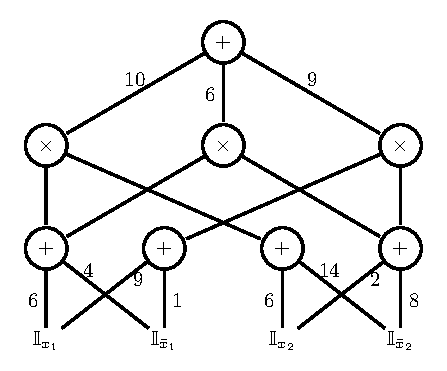
\includegraphics[width=0.5\textwidth]{SPN-example.pdf}
        \end{center}

        \cmuRedB{SPN Parameter Learning}
        \begin{itemize}
        \item The \cmuRed{parameters} are weights of the sum nodes.
        \item \cite{poon2011sum,gens2012discriminative} propose both
          \cmuRed{generative and discriminative} learning algorithms.
          These methods don't exploit the probabilistic properties embedded in the
          structure of the networks.
        \item \cite{peharz2015foundations} learn SPN parameters with
          the maximum likelihood principle by viewing them as
          \cmuRed{generative probabilistic models.}
          Such approaches often suffer from
          severe overfitting problems if the SPNs contain millions of parameters
          while the training data at hand only scales to tens of thousands.
        \end{itemize}

      \end{block}


    \end{column} % End of the first column

    % \begin{column}{\sepwid}\end{column}
    \hspace{-12cm}

    \begin{column}{\onecolwid}
      \begin{block}{Our Results}
        \cmuRedB{Variational Bayes Expectation Maximization}
        \begin{itemize}
        \item View the SPN $S$ as a \cmuRed{generative model} with $N$
          observable
          variables and $M$ hidden variables.
        \item Use a \cmuRed{Dirichlet prior} over the hidden variables
        \item View the SPN as a Bayesian network. Then with iid data,
          the likelihood function of $S$
          $\mathcal{L}(\Theta, x_{1:D})$ can me computed in
          $\mathcal{O}(D\abs{S})$, where $\abs{S}$ in the number of
          nodes and edges in the SPN.
        \item The exact posterior distribution over $\Theta$ is
          $p(\Theta|x_{1:D}) \propto p(\Theta)\mathcal{L}(\Theta|x_{1:D})$.
          This is a mixture of $\mathcal{O}(2^{MD})$ components
          that is intractable to compute and maintain exactly.
        \end{itemize}

        \cmuRedB{Sum-Product Networks as Mixture Models}

        \begin{itemize}
        \item \cmuRedB{Definition:}
          Given an SPN $\mathcal{S}$ over $x_{1:N}$,
          an \cmuRed{induced SPN} $\mathcal{T}$ with
          notes $\mathcal{T}_V$ and edges $\mathcal{T}_E$:
          \begin{itemize}
          \item Is an SPN over $x_{1:N}$.
          \item ${\rm Root(S)} \in \mathcal{T}_V$
          \item For all $v\in \mathcal{T}_V$, if $v$ is a sum node,
            then exactly one child of $v$ in $\mathcal{S}$ is in $\mathcal{T}_V$,
            with the corresponding edge in $\mathcal{T}_E$.
          \item If $v$ is a product node, then all the children
            of $v$ in $\mathcal{S}$ are in $\mathcal{T}_V$ and
            the corresponding edges are in $\mathcal{T}_E$.
          \end{itemize}
        \item Use induced SPNs to view the SPN as an \cmuRed{ensemble of trees}
          and can be treated as a mixture model with $\tau\ll 2^M$ effective
          components.
        \item The \cmuRed{exact posterior} is a mixture of $\tau^D$
          components
        \item Use variational methods to \cmuRed{approximate} the exact posterior
          by with a Dirichlet distribution by
          \cmuRed{minimizing the KL-divergence} between
          the approximate and exact posteriors.
          This minimization \cmuRed{is tractable} due to decomposability.
        \end{itemize}

        \cmuRedB{Optimization Problem}
        \begin{equation*}
          \argmin_\alpha \sum_{m=1}^M KL(q(\theta_m|\alpha_m) || \Pr(\theta_m|\alpha_m^0))
          - \log \Pr(X | \EE_{q(\Theta|\alpha)}[\Theta]),
        \end{equation*}
        where associated with each hidden variable $H_m$ are the
        the sum weights $\theta_m$, Dirichlet prior parameters $\alpha_m^0$,
        and Dirichlet posterior parameters $\alpha_m$.
        $\Theta = \theta_1 \ldots \theta_M$ and
        $$\EE_{q(\theta_m|\alpha_m)}[\theta_m] _i =
        {\alpha_{m,i} \over \sum_j \alpha_{m,j}}.$$

        This optimization problem has the intuitive interpretation
        using the KL divergence as a regularization term
        and the NLL as a data fitting term.
        Minimize this problem with gradient descent because
        the derivatives with respect to $\alpha$ have closed-form solutions.

      \end{block}
    \end{column}

    % \begin{column}{\sepwid}\end{column} % Empty spacer column
    \hspace{-12cm}
    \begin{column}{\onecolwid} % The third column
      \begin{block}{Empirical Results}
		\cmuRedB{Comparison with Projected Gradient Descent}
		\begin{table}
\centering
\begin{tabular}{|l||r|r|r|r|r|r|}\hline
\textbf{Data set} & $N$ & $|\mathcal{S}|$ & $D$ & Train & Valid & Test \\\hline
NLTCS & 16 & 13,733 & 1,716 & 16,181 & 2,157 & 3,236 \\
Retail & 135 & 56,931 & 22,113 & 22,041 & 2,938 & 4,408\\
MSWeb & 294 & 68,853 & 20,346 & 29,441 & 3,270 & 5,000 \\
\hline
\end{tabular}
\end{table}
\begin{figure}
\centering
	\begin{subfigure}[b]{0.3\textwidth}
		\centering
		\includegraphics[width=\textwidth]{nltcs-copts.pdf}
	\end{subfigure}
	~
	\begin{subfigure}[b]{0.3\textwidth}
		\centering
		\includegraphics[width=\textwidth]{tretail-copts.pdf}
	\end{subfigure}
	~
	\begin{subfigure}[b]{0.3\textwidth}
		\centering
		\includegraphics[width=\textwidth]{msweb-copts.pdf}
	\end{subfigure}
\end{figure}

\begin{table}
\begin{subtable}[b]{0.45\linewidth}
\centering
\caption{Test set avg log-likelihood.}
\begin{tabular}{|l||r|r|r|}\hline
\textbf{Data set} & PGD & VBEM \\\hline
NLTCS & -6.43534 & \textbf{-6.07951} \\
Retail & -15.5319 & \textbf{-10.8977}  \\
MSWeb & -19.6908 & \textbf{-9.84271} \\\hline
\end{tabular}
\end{subtable}%
\begin{subtable}[b]{0.45\linewidth}
\centering
\caption{Training time (sec).}
\begin{tabular}{|l||r|r|r|}\hline
\textbf{Data set} & PGD & VBEM \\\hline
NLTCS & \textbf{521.9}  & 795.1 \\
Retail & 26196.8 & \textbf{13236.7} \\
MSWeb & \textbf{12840.4} & 23445.6\\\hline
\end{tabular}
\end{subtable}
\end{table}
      \end{block}

      \begin{block}{Conclusions}
        \begin{itemize}
        \item 	We present a \cmuRed{tractable Bayesian inference algorithm} of Sum-Product Networks. 
        \item 	We convert the Bayesian inference problem into an optimization problem by using collapsed variational method. 
        \end{itemize}
      \end{block}

      \begin{block}{References}
        {\small
          \bibliographystyle{alpha}
          \bibliography{refs}
        }
      \end{block}

    \end{column} % End of the third column

  \end{columns} % End of all the columns in the poster

\end{frame} % End of the enclosing frame

\end{document}
